\sectionframe{Period-adding-like Structures in the Archetypal Model}
\section{Period-adding-like}

\begin{frame}{Configuration Changes}
	\vspace{-1em}
	\begin{figure}
		\includegraphics[width=.3 \textwidth]{60_MinimalRepr/Cobweb_E16/result.png}
		\quad
		\includegraphics[width=.3 \textwidth]{62_MinimalRepr_Adding/Cob_1_ZCorn/result.png}
	\end{figure}
	\vspace{1em}
	Got rid of the local minima on branches $f_\A$ and $f_\C$
\end{frame}

\begin{frame}{Period-adding-like Structures in the Archetypal Model}
	\begin{figure}
		\includegraphics[width=.4 \textwidth]{62_MinimalRepr_Adding/2D_Regions_1/Manual/result.png}
		\quad
		\includegraphics[width=.4 \textwidth]{62_MinimalRepr_Adding/2D_Period_add_zoom/result.png}
	\end{figure}
\end{frame}

%\begin{frame}{Changes to the Bifurcation Structure}
%	\begin{itemize}
%		\item ``Type B'' parameter regions disappeared
%		\item ``Type A'' parameter regions of the same chains start overlapping
%		      \pause
%		\item New space in-between chains
%	\end{itemize}
%\end{frame}

\begin{frame}{Describing the Period-adding-like Structures}
	\vspace{-1em}
	\begin{figure}
		\only<1>{
			\includegraphics[width=.4 \textwidth]{62_MinimalRepr_Adding/2D_Period_add_zoom_hor/result.png}
			\qquad
			\includegraphics[width=.4 \textwidth]{../Figures/7/7.12b/result.png}
		}
		\only<2>{
			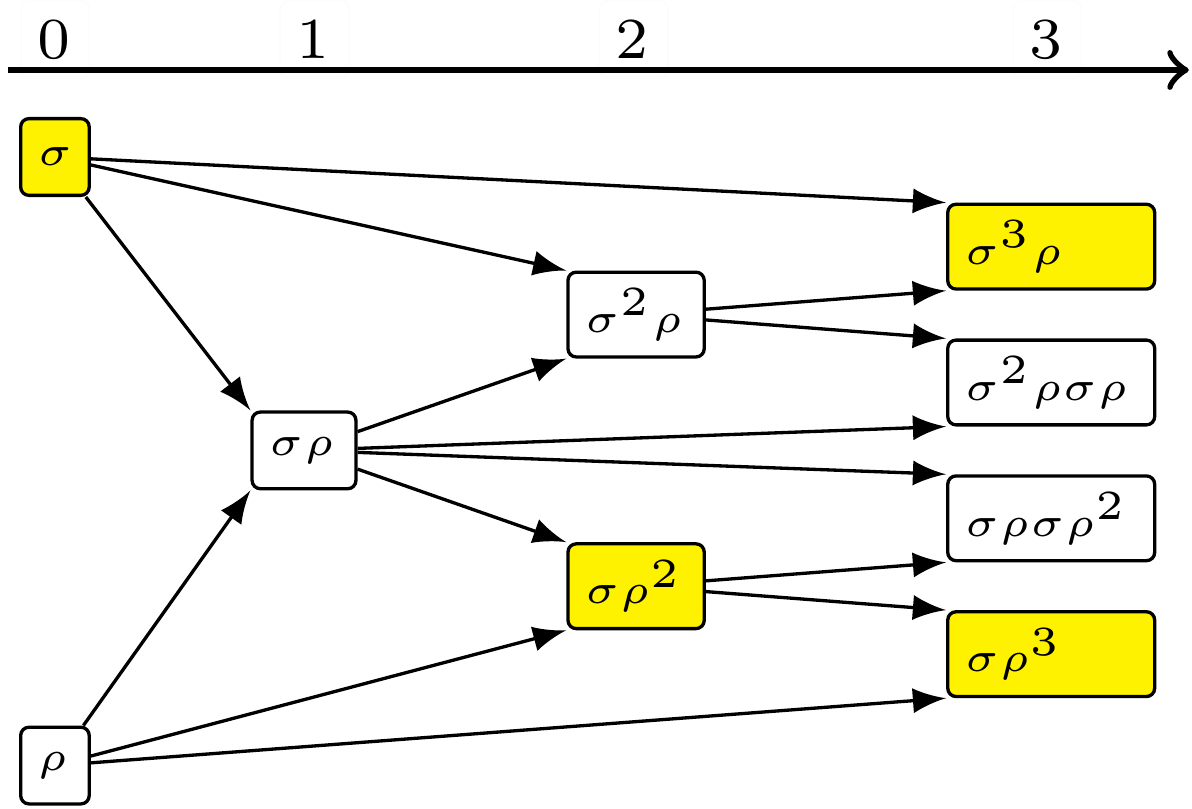
\includegraphics[width=.7 \textwidth]{../Figures/7/7.13/adding.png}
		}
	\end{figure}
\end{frame}

\begin{frame}{Result of Describing the Structures}
	This is not period-adding
	\begin{itemize}
		\item Periods don't add
		\item Symbolic sequences don't concatenate
	\end{itemize}
	\vspace{1em}
	But it is similar
\end{frame}
